
%     Copyright 2021, Abt Dávid Ottó

%         Szegedi Tudományegyetem
% Természettudományi és Informatikai Kar
%          Informatikai tanszék

% A szakdolgozathoz felhasználtam az alábbi linkeken található sablont:
% https://github.com/szledan/thesis-template

\documentclass[12pt,numbers=noenddot]{report}

\usepackage[a4paper]{geometry}
\usepackage{lmodern}			% Kijelölhető az összes karakter
\usepackage[utf8]{inputenc}		% Ékezetes szavak beviteléhez
\usepackage[hungarian]{babel}	% Magyar nyelv támogatása
\usepackage{fontspec}			% Fontok támogatása
\setmainfont{Nimbus Roman}		% FOSS Times New Roman alternatíva
\usepackage{titlesec}			% Fejlécben lévő cím margójának beállítására
\usepackage{fancyhdr}			% Fej- és láblécek személyreszabása
\usepackage{graphicx}			% Képek
\graphicspath{ {./img/} }
\usepackage{color}				% Színek
\usepackage{xcolor}				% -||-
\usepackage{subfig}
\usepackage{caption}
\captionsetup[figure]{labelsep=colon}
\usepackage{tikz}
\usepackage{float}				% Hogy az ábrák a helyükön maradjanak
\usepackage{wrapfig}			% Kép mellett folyó íráshoz
\usepackage{listings}			% Forráskódok
\usepackage{lastpage}			% Utolsó oldal száma
\usepackage[unicode]{hyperref}	% Linkek
\hypersetup{
	colorlinks,
	citecolor=black,
	filecolor=black,
	linkcolor=black,
	urlcolor=black
}
\usepackage[block=ragged]{biblatex}
\BiblatexHungarianWarningOff
\bibliography{cites}
\DeclareFieldFormat{urldate}{Látogatás:}

\usepackage{amsmath}

\usepackage{multicol}

% Egyéni színek
\definecolor{codegreen}{rgb}{0,0.6,0}
\definecolor{codegray}{rgb}{0.5,0.5,0.5}
\definecolor{codepurple}{rgb}{0.58,0,0.82}
\definecolor{backcolour}{rgb}{0.95,0.95,0.92}

% Kódrészletek
\lstset{ %
	backgroundcolor=\color{backcolour},
	commentstyle=\color{codegreen},
	keywordstyle=\color{magenta},
	numberstyle=\tiny\color{codegray},
	stringstyle=\color{codepurple},
	basicstyle=\ttfamily\footnotesize,
	breakatwhitespace=false,
	breaklines=true,
	captionpos=b,
	keepspaces=true,
	numbers=left,
	numbersep=5pt,
	showspaces=false,
	showstringspaces=false,
	showtabs=false,
	tabsize=4,
	extendedchars=true
}

% Ábrák számozása
\renewcommand{\thefigure}{\arabic{chapter}.\arabic{figure}}
% Ábrák "ábra" felirata
\addto\captionsmagyar{\renewcommand{\figurename}{{\'a}bra}}

% Tartalomjegyzék elemeinek számozása:
\setcounter{tocdepth}{3}
\setcounter{secnumdepth}{3}

% Margók:
\voffset	-1in
\textwidth	150mm
\topmargin	15mm
\headheight	10mm
\headsep	5mm
\textheight	237mm

% A Word-ös 1.5-ös sorköznek ez felel meg
\linespread{1.25}

\begin{document}

\pagestyle{fancyplain}
\fancyhf{}
\renewcommand{\headrulewidth}{0pt}	% Eltűnteti a fejlécben lévő vonalat

\titleformat{\chapter}[display]
{\normalfont\huge\bfseries}{\thechapter. \chaptertitlename}{20pt}{\Huge}
\titlespacing*{\chapter}{0pt}{0pt}{40pt}

\newcommand{\szerzo}{Abt Dávid Ottó}
\newcommand{\cim}{Másodrendű sajátvektor centralitások vizsgálata}

%%%%%%%%%%%%%%%%%%%%%%%%%%%%%%%%%%%%%%%%%%%%%%%%%%%%%%%%%%%%%%%%%%%%%%%%%%%%%%%%
%% Elülső kötéstábla                                                          %%
%%%%%%%%%%%%%%%%%%%%%%%%%%%%%%%%%%%%%%%%%%%%%%%%%%%%%%%%%%%%%%%%%%%%%%%%%%%%%%%%

\newpage
\thispagestyle{empty}
\fancyfoot[C]{}	% Lábléc eltüntetése

\begin{center}

	\vspace*{2cm}

	{\Large\bf Szegedi Tudományegyetem}

	\vspace{.5cm}

	{\Large\bf Informatikai Intézet}

	\vspace*{8.5cm}

	{\Huge\bf SZAKDOLGOZAT}

	\vspace*{7cm}

	{\LARGE\bf \szerzo}

	\vspace*{.6cm}

	{\Large\bf 2022}

\end{center}

%%%%%%%%%%%%%%%%%%%%%%%%%%%%%%%%%%%%%%%%%%%%%%%%%%%%%%%%%%%%%%%%%%%%%%%%%%%%%%%%
%% Címlap                                                                     %%
%%%%%%%%%%%%%%%%%%%%%%%%%%%%%%%%%%%%%%%%%%%%%%%%%%%%%%%%%%%%%%%%%%%%%%%%%%%%%%%%

\newpage
\thispagestyle{plain}

\begin{center}
	\vspace*{.6cm}

	{\Large\bf Szegedi Tudományegyetem}

	\vspace{.5cm}

	{\Large\bf Informatikai Tanszékcsoport}

	\vspace*{3.5cm}

	{\LARGE\bf \cim}

	\vspace*{3.2cm}

	{\Large Szakdolgozat}

	\vspace*{3.5cm}

	\large
	\begin{tabular}{c@{\hspace{4cm}}c}
	\emph{Készítette:}						&\emph{Témavezető:}\\
	\textbf{\szerzo}						&\textbf{Dr. Vinkó Tamás}\\
	programtervező informatikus BSc				&egyetemi docens\\
	hallgató								&
	\end{tabular}

	\vspace*{3.5cm}

	\Large {
		Szeged\\
		\vspace{2mm}
		2022
	}
\end{center}

%%%%%%%%%%%%%%%%%%%%%%%%%%%%%%%%%%%%%%%%%%%%%%%%%%%%%%%%%%%%%%%%%%%%%%%%%%%%%%%%
%% Üres oldal                                                                 %%
%%%%%%%%%%%%%%%%%%%%%%%%%%%%%%%%%%%%%%%%%%%%%%%%%%%%%%%%%%%%%%%%%%%%%%%%%%%%%%%%

\newpage
\thispagestyle{plain}
\mbox{}

%%%%%%%%%%%%%%%%%%%%%%%%%%%%%%%%%%%%%%%%%%%%%%%%%%%%%%%%%%%%%%%%%%%%%%%%%%%%%%%%
%% Feladatkiírás                                                              %%
%%%%%%%%%%%%%%%%%%%%%%%%%%%%%%%%%%%%%%%%%%%%%%%%%%%%%%%%%%%%%%%%%%%%%%%%%%%%%%%%

\chapter*{Feladatkiírás}
\setcounter{page}{1}	% A lapszámláló újrainicializálása
\fancyfoot[R]{\thepage}
\addcontentsline{toc}{section}{Feladatkiírás}

Elterjedt hobbi az operációs rendszer, illetve kernel fejlesztése az olyan
programozók közt, akik szeretnének többet megtudni a számítógépek működéséről.
Ennek köszönhetően az interneten számos nyílt forráskódú hobbi operációs
rendszerrel, valamint az azok írásához felhasználható útmutatókkal
találkozhatunk. Sajnálatos módon ezen leírások nagy része elavult, túl
bonyolult, vagy nem elég részletes ahhoz, hogy egy kezdő bármit is megértsen
belőle, ezért elhatároztam, hogy megírok egy jól dokumentált, egyszerűen
használható és bővíthető operációs rendszert, és kialakítok hozzá egy gyorsan
felállítható fejlesztői környezetet, amelynek beüzemelése mindössze pár parancs.

\hfill \break
A feladat része, hogy az operációs rendszer rendelkezzen a legszükségszerűbb
alap funkciókkal, és tartalmazzon pár programot és/vagy játékot is.

%%%%%%%%%%%%%%%%%%%%%%%%%%%%%%%%%%%%%%%%%%%%%%%%%%%%%%%%%%%%%%%%%%%%%%%%%%%%%%%%
%% Tartalmi összefoglaló                                                      %%
%%%%%%%%%%%%%%%%%%%%%%%%%%%%%%%%%%%%%%%%%%%%%%%%%%%%%%%%%%%%%%%%%%%%%%%%%%%%%%%%

\chapter*{Tartalmi összefoglaló}
\addcontentsline{toc}{section}{Tartalmi összefoglaló}

\subsubsection*{A téma megnevezése}

\cim

\subsubsection*{A megadott feladat megfogalmazása}

A feladat egy olyan operációs rendszer megírása, amely bootolás után egy
egyszerű parancssori, illetve grafikus felhasználói felületet biztosít, és
emellett rendelkezik néhány programmal és játékkal is.

\subsubsection*{A megoldásmód}

Az egyszerűség kedvéért az összes program a kernelbe van "égetve", és
kernelszintű hozzáférése van, valamint néhány olyan elem megvalósításához,
amely nem része a feladatkiírásnak, és túl sok időbe telt volna egy működő
implementáció feltalálása, már létező nyílt forráskódú és szabad szoftverek
részeit portoltam le, vagy azok működési elvei alapján írtam meg a saját
implementációmat.

\subsubsection*{Alkalmazott eszközök, módszerek}

A fejlesztés a \textit{VSCodium} és \textit{Vim} szövegszerkesztők segítségével
zajlott C, C++ és 32-bites x86 assembly nyelven.
A szoftver fordítására a \textit{gcc, g++, gas} fordítókat, hibakereséshez
\textit{GDB}-t, virtualizációhoz pedig nagyrészt \textit{QEMU}-t, majd később az
\textit{Oracle VirtualBox}-ot használtam. A build folyamatokat a
\textit{GNU Make} szoftver segítségével automatizálam.

\subsubsection*{Elért eredmények}

Az operációs rendszerem sikeresen bootol virtuális gépeken, és a tesztelt
funkciók hiba nélkül működnek.

\subsubsection*{Kulcsszavak}

operációs rendszer, kernel, bootloader, GRUB, Intel, x86, QEMU, VirtualBox

%%%%%%%%%%%%%%%%%%%%%%%%%%%%%%%%%%%%%%%%%%%%%%%%%%%%%%%%%%%%%%%%%%%%%%%%%%%%%%%%
%% Tartalomjegyzék                                                            %%
%%%%%%%%%%%%%%%%%%%%%%%%%%%%%%%%%%%%%%%%%%%%%%%%%%%%%%%%%%%%%%%%%%%%%%%%%%%%%%%%

\renewcommand{\contentsname}{Tartalomjegyzék}
\tableofcontents

%%%%%%%%%%%%%%%%%%%%%%%%%%%%%%%%%%%%%%%%%%%%%%%%%%%%%%%%%%%%%%%%%%%%%%%%%%%%%%%%
%% Bevezetés                                                                  %%
%%%%%%%%%%%%%%%%%%%%%%%%%%%%%%%%%%%%%%%%%%%%%%%%%%%%%%%%%%%%%%%%%%%%%%%%%%%%%%%%

\chapter{Bevezetés}
\addcontentsline{toc}{section}{Bevezetés}
\pagestyle{fancy}

Manapság körbevesznek minket a számítógépek, és életünk nélkülözhetetlen részévé
váltak. Már gyerekkorom óta számítógépek közt nevelkedtem, mégis úgy éreztem,
hogy nem tudok róluk eleget. Gimnáziumi éveim alatt olvastam egy cikket egy
Terry Davis nevű programozóról, aki a saját operácios rendszerének
fejlesztésére szentelte az életét. Mivel mindig is érdekelt a számítógépek
működése, a cikk hatására elolvastam pár útmutatót arról, hogy hogyan írhanék
otthon egy saját operációs rendszert. Az egyik ilyen útmutatót követve el is
kezdtem a fejlesztést, azonban a nehézségek miatt hamar feladtam.

Egészen az egyetem második évéig nem rendelkeztem sem elegendő tudással,
kitartással, sem pedig idővel egy ekkora méretű projekthez. Ekkor a nyári
szünetben kezdtem újra a projektet, és a szakdolgozattal beadott "végleges"
verzió befejezéséig csaknem másfél év telt el, ezalatt folyamatosan
fejlesztettem.

Az operációs rendszeremet második kutyám (Rex) után RexOS-re kereszteltem. A
fejlesztés és a tanulás során azt vettem észre, hogy a legtöbb operációs
rendszerek, illetve kernelek fejlesztéséhez való útmutató elavult információkkal
szolgál, vagy nehezen érthető egy kezdő számára, és sokszor a kódrészletek
hibásak / hiányosak, vagy pedig egyáltalán nincs is kódrészlet, ami segítené
egy-egy folyamat működésének megértését.
Ezek a nehézségek vettek rá, hogy a projektemben ügyeljek a kód átláthatóságára
és arra, hogy jól legyen dokumentálva, illetve hogy mindenki számára elérhető
legyen, ezzel segítve a hobbi operációs rendszerek fejlesztőit.

A 32-bites Intel architektúra mellett döntöttem, mert ehhez találtam a legtöbb
forrásanyagot, így a fejlesztése könnyebbnek bizonyult, mint egy 64-bites
operációs rendszeré. Eredetileg az is szerepelt a céljaim közt, hogy
lehessen valós hardveren futtatni, azonban erről lemondtam, amikor megtudtam,
hogy a mai számítógépek nem támogatják a VGA mode 3-at, amit az operációs
rendszerem a tartalom megjelenítésére használ, valamint a VESA VBE-t támogató
hardware is egyre ritkább.

%%%%%%%%%%%%%%%%%%%%%%%%%%%%%%%%%%%%%%%%%%%%%%%%%%%%%%%%%%%%%%%%%%%%%%%%%%%%%%%%
%% Alapfogalmak                                                                  %%
%%%%%%%%%%%%%%%%%%%%%%%%%%%%%%%%%%%%%%%%%%%%%%%%%%%%%%%%%%%%%%%%%%%%%%%%%%%%%%%%

\chapter{Alapfogalmak}
\addcontentsline{toc}{section}{Bevezetés}
\pagestyle{fancy}

\section{Gráf}

Egy gráf definiálható egy $G=(V,E)$ párként, ahol V a gráf csúcsainak, E az éleinek halmaza. Az E halmaz V-beli elempárokat tartalmaz. 
($E \subseteq V \times V$)

Ez a matematikai struktúra alkalmas különböző entitások közti bináris kapcsolatok tárolására. Ezek lehetnek akár egy szociális médiai platform felhasználói közti ismerettségek, vagy egy internetes enciklopédia kulcsszavai közti összefüggések. A gráfok ezen tulajdonságát használja ki például a \textit{neo4j} nevű gráf adatbázis kezelő rendszer is.

\section{Mátrix}
A mátrix egy kétdimenziós listaként képzelhető el, ami nem csupán egy $m * n$ elemet tároló struktúra, hanem az elemek elhelyezkedésének köszönhetően jóval több információt tárol mint egy $m * n$ elemű halmaz.

\section{Gráf ábrázolások, mátrix}
A gráfokat ábrázolására a két legnépszerűbb adatszerkezet a szomszédsági lista, illetve a szomszédsági mátrix.

A másodrendű sajátvektor centralitások vizsgálatához a szomszédsági mátrixokat fogjuk használni, mivel mátrixokon jóval könnyebb az ezekhez szükséges műveleteket elvégezni mint láncolt listákon.

A szomszédsági mátrix egy $n \times n$-es mátrix, ahol $n$ a gráf csúcsainak száma. Az $m$-edik sor $n$-edik eleme megadja, hogy a gráf $m$-edik és $n$-edig csúcsa közt vezet-e él.


\pagebreak

\section{Sajátérték, sajátvektor}
A mátrixokat felfoghatjuk egy geometriai transzformációként amit egy vektoron végzünk el. Például az $\textbf{A}$ mátrix a $\vec{v}$ vektort az alábbiak szerint módosítja:

$$
\textbf{A} \vec{v} = \vec{w}
$$

$$
{
	\begin{bmatrix}
		a & b \\
		c & d \\
	\end{bmatrix}
}
{
	\begin{bmatrix}
		x \\
		y \\
	\end{bmatrix}
}
=
{
	\begin{bmatrix}
		a*x+b*y \\
		c*x+d*y \\
	\end{bmatrix}
}
$$

\vspace{1cm}

A transzformáció irányát és mértékét a sajátvektor és a sajátérték jellemzi.
Definíció szerint $A$ mátrix $v$ sajátétvektora és $\lambda$ sajátértéke közt az összefüggés: $$A \lambda = v \lambda$$


\section{Centralitás}
A gráfok atomi tulajdonságain (pl.: van-e él két csúcs között) kívül sok értékes információ kinyerhető különböző metrikákkal. 
Például a csúcsok "fontosságának" egy kimutatására szolgálnak a centralitások, amik egy sorrendet képeznek a gráf pontjai közt. 

A legegyszerűbb centralitás a fokszám centralitás, ami az adott csúcs fokszáma szerint képez sorrendet.


\noindent
\begin{minipage}[c]{0.4\linewidth}

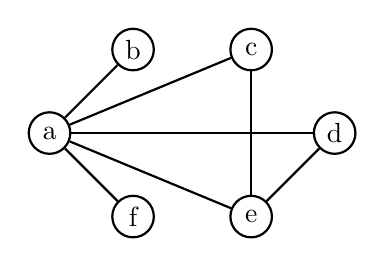
\begin{tikzpicture}[node distance=15mm, inner sep=0pt, minimum size=15pt, thick, main/.style = {draw, circle}]
	\node[main] (1) {a};
	\node[main] (2) [above right of=1] {b};
	\node[main] (3) [right of=2] {c}; 
	\node[main] (4) [below right of=3] {d};
	\node[main] (5) [below left of=4] {e}; 
	\node[main] (6) [left of=5] {f};
	\draw (1) -- (2);
	\draw (1) -- (3);
	\draw (1) -- (4);
	\draw (1) -- (5);
	\draw (1) -- (6);
	\draw (3) -- (5);
	\draw (4) -- (5);
\end{tikzpicture}

\end{minipage}
% \columnbreak
\noindent
\begin{minipage}[c]{0.2\linewidth}

\hspace{0.5cm}
$\rightarrow$

\end{minipage}
% \columnbreak
\begin{minipage}[c]{0.2\linewidth}

\begin{align}
	\begin{bmatrix}
		deg(a)\\
		deg(b)\\
		deg(c)\\
		deg(d)\\
		deg(e)\\
		deg(f)
	\end{bmatrix}
	=
	\begin{bmatrix}
		5\\
		1\\
		2\\
		2\\
		3\\
		1
	\end{bmatrix}
\end{align}

\end{minipage}

\vspace{0.5cm}

A ábrán szereplő 6 pontú gráfhoz egy 6 hosszúságú vektort rendelt, melynek elemei az egyes csúcsok fokszámával egyeznek meg.

A fokszám centralitás kiszamítható gráfot leíró $n \times n$ szomszédsági mátrix valamint egy $n$ elemű, egyesekből álló vektor szorzataként:

\begin{align}
	\begin{bmatrix}
		0 & 1 & 1 & 1 & 1 & 1 \\
		1 & 0 & 0 & 0 & 0 & 0 \\
		1 & 0 & 0 & 0 & 1 & 0 \\
		1 & 0 & 0 & 0 & 1 & 0 \\
		1 & 0 & 1 & 1 & 0 & 0 \\
		1 & 0 & 0 & 0 & 0 & 0 \\
	\end{bmatrix}
	*
	\begin{bmatrix}
		1\\
		1\\
		1\\
		1\\
		1\\
		1
	\end{bmatrix}
	=
	\begin{bmatrix}
		5\\
		1\\
		2\\
		2\\
		3\\
		1
	\end{bmatrix}
\end{align}



%%%%%%%%%%%%%%%%%%%%%%%%%%%%%%%%%%%%%%%%%%%%%%%%%%%%%%%%%%%%%%%%%%%%%%%%%%%%%%%%
%% Fejlesztői környezet                                                       %%
%%%%%%%%%%%%%%%%%%%%%%%%%%%%%%%%%%%%%%%%%%%%%%%%%%%%%%%%%%%%%%%%%%%%%%%%%%%%%%%%

\chapter{Fejlesztői környezet}

A szoftver fejlesztése GNU+Linux operációs rendszeren zajlott, az alábbiakban
olvasható a felhasznált szoftverek összessége, és azoknak a felhasználási módja.

%%%%%%%%%%%%%%%%%%%%%%%%%%%%%%%%%%%%%%%%%%%%%%%%%%%%%%%%%%%%%%%%%%%%%%%%%%%%%%%%
%% VSCodium                                                                   %%
%%%%%%%%%%%%%%%%%%%%%%%%%%%%%%%%%%%%%%%%%%%%%%%%%%%%%%%%%%%%%%%%%%%%%%%%%%%%%%%%

\section{Visual Studio Codium}

A kód írásához a Microsoft Visual Studio Code nyílt forráskódú és szabad
változatát, a VSCodium-ot használtam. Telepítve volt a Microsoft C/C++
bővítménye mellett az \textit{ASM Code Lens} az assembly forrásfájlok
szintaxisának a kiemelése miatt, illetve a
\textit{Doxygen Documentation Generator} nevű bővítményt a dokumentáció
automatikus generálásához.

%%%%%%%%%%%%%%%%%%%%%%%%%%%%%%%%%%%%%%%%%%%%%%%%%%%%%%%%%%%%%%%%%%%%%%%%%%%%%%%%
%% GNU Make                                                                   %%
%%%%%%%%%%%%%%%%%%%%%%%%%%%%%%%%%%%%%%%%%%%%%%%%%%%%%%%%%%%%%%%%%%%%%%%%%%%%%%%%

\section{GNU Make}

A build folyamatok automatizálásához a GNU Make-et használtam. Minden egyes
nyelv forrásfájljait külön make targetekbe csoportosítottam, illetve az initrd,
és a bootolható iso fájl is külön targetet kapott.

\begin{verbatim}
HDRS := $(shell find $(SRC_DIR) -regex ".*\.\(hpp\|h\|inc\)")
SRCS := $(shell find $(SRC_DIR) -regex ".*\.\(cpp\|c\|S\)")
OBJS := $(SRCS:%=$(BUILD_DIR)/%.o)
\end{verbatim}

\noindent A fenti sorok begyűjtik az összes fejlécet és forrásfájlt egy-egy
listába, az alábbiakban látható a C forrásfájlok targetje:

\begin{verbatim}
$(BUILD_DIR)/%.c.o: %.c $(HDRS)
    @mkdir -p $(dir $@)
    @$(PROGRESS) && echo "Processing C source file: $<"
    @$(CC) $(CFLAGS) -c $< -o $@
\end{verbatim}

\noindent Ügyeltem arra, hogy a fordító 32-bites rendszerre kompiláljon, és a C
és C++ forrásfájlok esetén a standard könyvtárak helyett az én implementációmat
használja.


%%%%%%%%%%%%%%%%%%%%%%%%%%%%%%%%%%%%%%%%%%%%%%%%%%%%%%%%%%%%%%%%%%%%%%%%%%%%%%%%
%% Konklúzió                                                                  %%
%%%%%%%%%%%%%%%%%%%%%%%%%%%%%%%%%%%%%%%%%%%%%%%%%%%%%%%%%%%%%%%%%%%%%%%%%%%%%%%%

\chapter{Konklúzió}

A QEMU-ban, illetve VirtualBox-ban végrehajtott tesztelés összességében sikerrel
zajlott. Az alábbiakban részletezem a tesztelt funkciókat, és a kapott
eredményt.

\hfill \break
Végrehajtott tesztek:

\begin{enumerate}
	\item Bootolás QEMU-ban és VirtualBox-ban- sikeres
	\item Megszakítások - működnek
	\item PCI - kilistázza az összes PCI sínnel csatlakoztatott perifériát
	\item Fájlrendszer - felismeri a FAT32-es elsődleges partíciókat, és
	működik a fájlok tartalmának olvasása is
	\item Hálózat (VirtualBox) - működik a kommunikáció a számítógépen nyitott
	netcat-tel, illetve Android eszközön futtatott Debianon lévő netcat-tel is
	\item Soros port (QEMU) - bootoláskor kiírja a boot logot a standard
	outputra, illetve standard inputra bevitt karakterek megjelennek RexOS-en
	\item Párhuzamos port (QEMU) - kiírja a kívánt szöveget
	\item Játékok - hiba nélkül működnek
\end{enumerate}

\noindent Nem lett letesztelve:

\begin{enumerate}
	\item Hálózat (QEMU)
	\item Soros, illetve párhuzamos port (VirtualBox)
	\item Valós hardveren bootolás
\end{enumerate}

\noindent Az operációs rendszerem fejlesztése során rengeteg új információt,
tudást sajátítottam el, és sikerült közelebb kerülnöm a számítógépek működésének
megértéséhez.

%%%%%%%%%%%%%%%%%%%%%%%%%%%%%%%%%%%%%%%%%%%%%%%%%%%%%%%%%%%%%%%%%%%%%%%%%%%%%%%%
%% Irodalomjegyzék                                                            %%
%%%%%%%%%%%%%%%%%%%%%%%%%%%%%%%%%%%%%%%%%%%%%%%%%%%%%%%%%%%%%%%%%%%%%%%%%%%%%%%%

\clearpage
\phantomsection
\addcontentsline{toc}{section}{Irodalom}

\printbibliography

%%%%%%%%%%%%%%%%%%%%%%%%%%%%%%%%%%%%%%%%%%%%%%%%%%%%%%%%%%%%%%%%%%%%%%%%%%%%%%%%
%% Nyilatkozat                                                                %%
%%%%%%%%%%%%%%%%%%%%%%%%%%%%%%%%%%%%%%%%%%%%%%%%%%%%%%%%%%%%%%%%%%%%%%%%%%%%%%%%

\chapter*{Nyilatkozat}
\addcontentsline{toc}{section}{Nyilatkozat}

Alulírott \szerzo, Programtervező Informatikus hallgató, kijelentem,
hogy a dolgozatomat a Szegedi Tudományegyetem, Informatikai Tanszékcsoport
Szoftverfejlesztési Tanszékén készítettem, alapszakos diploma megszerzése
érdekében.

\hfill \break
Kijelentem, hogy a dolgozatot más szakon korábban nem védtem meg, saját munkám
eredménye, és csak a hivatkozott forrásokat (szakirodalom, eszközök, stb.)
használtam fel.

\hfill \break
Tudomásul veszem, hogy szakdolgozatomat a Szegedi Tudományegyetem
Informatikai Tanszékcsoport könyvtárában, a helyben olvasható könyvek között
helyezik el.

\vspace*{2cm}

\begin{tabular}{lc}
Szeged, \today
\hspace{2cm} & \makebox[6cm]{\dotfill} \\
& aláírás \\
\end{tabular}

%%%%%%%%%%%%%%%%%%%%%%%%%%%%%%%%%%%%%%%%%%%%%%%%%%%%%%%%%%%%%%%%%%%%%%%%%%%%%%%%
%% Köszönetnyilvánítás                                                        %%
%%%%%%%%%%%%%%%%%%%%%%%%%%%%%%%%%%%%%%%%%%%%%%%%%%%%%%%%%%%%%%%%%%%%%%%%%%%%%%%%

\chapter*{Köszönetnyilvánítás}
\addcontentsline{toc}{section}{Köszönetnyilvánítás}

Szeretném megköszönni a hasznos ismertetőket és kódrészleteket az
\textbf{OSDev wiki szerkesztőinek}, illetve az \textbf{OSDev Discord
szerver tagjainak} útbaigazításait, \textbf{James Molloynak} a kiváló
leírásokkal teli weboldalát, az érthető és szórakoztató
\textit{Write your own Operating System} c. videósorozatot pedig
\textbf{Viktor Engelmannak}. Ez a YouTube videósorozat rengeteget segített nekem
a fejlődésben és az operációs rendszerek működésének megértésében. Egyúttal
szeretném megköszönni a segítségét minden ismerősömnek, aki részt vett az
operációs rendszerem tesztelésben.

\end{document}
